\documentclass[11pt]{article}\usepackage[]{graphicx}\usepackage[]{xcolor}
% maxwidth is the original width if it is less than linewidth
% otherwise use linewidth (to make sure the graphics do not exceed the margin)
\makeatletter
\def\maxwidth{ %
  \ifdim\Gin@nat@width>\linewidth
    \linewidth
  \else
    \Gin@nat@width
  \fi
}
\makeatother

\definecolor{fgcolor}{rgb}{0.345, 0.345, 0.345}
\newcommand{\hlnum}[1]{\textcolor[rgb]{0.686,0.059,0.569}{#1}}%
\newcommand{\hlstr}[1]{\textcolor[rgb]{0.192,0.494,0.8}{#1}}%
\newcommand{\hlcom}[1]{\textcolor[rgb]{0.678,0.584,0.686}{\textit{#1}}}%
\newcommand{\hlopt}[1]{\textcolor[rgb]{0,0,0}{#1}}%
\newcommand{\hlstd}[1]{\textcolor[rgb]{0.345,0.345,0.345}{#1}}%
\newcommand{\hlkwa}[1]{\textcolor[rgb]{0.161,0.373,0.58}{\textbf{#1}}}%
\newcommand{\hlkwb}[1]{\textcolor[rgb]{0.69,0.353,0.396}{#1}}%
\newcommand{\hlkwc}[1]{\textcolor[rgb]{0.333,0.667,0.333}{#1}}%
\newcommand{\hlkwd}[1]{\textcolor[rgb]{0.737,0.353,0.396}{\textbf{#1}}}%
\let\hlipl\hlkwb

\usepackage{framed}
\makeatletter
\newenvironment{kframe}{%
 \def\at@end@of@kframe{}%
 \ifinner\ifhmode%
  \def\at@end@of@kframe{\end{minipage}}%
  \begin{minipage}{\columnwidth}%
 \fi\fi%
 \def\FrameCommand##1{\hskip\@totalleftmargin \hskip-\fboxsep
 \colorbox{shadecolor}{##1}\hskip-\fboxsep
     % There is no \\@totalrightmargin, so:
     \hskip-\linewidth \hskip-\@totalleftmargin \hskip\columnwidth}%
 \MakeFramed {\advance\hsize-\width
   \@totalleftmargin\z@ \linewidth\hsize
   \@setminipage}}%
 {\par\unskip\endMakeFramed%
 \at@end@of@kframe}
\makeatother

\definecolor{shadecolor}{rgb}{.97, .97, .97}
\definecolor{messagecolor}{rgb}{0, 0, 0}
\definecolor{warningcolor}{rgb}{1, 0, 1}
\definecolor{errorcolor}{rgb}{1, 0, 0}
\newenvironment{knitrout}{}{} % an empty environment to be redefined in TeX

\usepackage{alltt}

% Packages for graphics & layout
\usepackage{graphicx}
\usepackage{epstopdf}
\usepackage{caption}
\usepackage{subcaption}
\usepackage{booktabs}
\usepackage[a4paper,margin=0.5in]{geometry}
\usepackage{lipsum}
\usepackage{multicol}

\usepackage[utf8]{inputenc}
\usepackage{enumitem}

% Packages for math
\usepackage{amsmath}
\usepackage{amsfonts}
\usepackage{amssymb}

% Package for bibliography
\usepackage{natbib}
\usepackage{hyperref}
hypersetup{
    colorlinks=true,      % Set to false to disable coloring links
    linkcolor=blue,       % Color of internal links
    filecolor=magenta,    % Color of file links
    urlcolor=cyan,        % Color of external links
    citecolor=green,      % Color of citations
    pdftitle={My Document Title},    % PDF document title
    pdfauthor={Author Name},         % PDF document author
    pdfsubject={Subject of the Document}, % PDF document subject
    pdfkeywords={keyword1, keyword2, keyword3}, % PDF document keywords
    bookmarksnumbered=true,         % If true, adds numbers to sections in PDF bookmarks
    bookmarksopen=true,             % If true, the PDF bookmarks are expanded by default
    bookmarksopenlevel=1,           % Level of bookmarks which are opened by default
    pdfstartview=Fit,               % Sets the default view of the PDF when opened
    pdfpagemode=UseOutlines,        % Determines how the PDF file is opened in Acrobat Reader
}
% listing setup \usepackage{listings}
\usepackage{color} % For syntax highlighting color
\captionsetup{labelfont=bf}
\setlength{\parskip}{0.5\baselineskip}


\title{\textbf{Data Analysis Report}}
\author{Michael V Cumbo}
\date{\today}
\IfFileExists{upquote.sty}{\usepackage{upquote}}{}
\begin{document}

\maketitle

\section{Introduction}
This paper was written in response to the United Auto Workers strike and the SAG-AFTRA strike of 2023. The goal of this paper is to contextualize the state of trade union power in the United States, blending data analysis with a literature review. The data in this paper will contextualize union power in a select number of nation-states, adding perspective to the modes of influence unions have.

\section{Methodology}
\subsection*{Libraries Used in the Analysis}

This analysis utilized several R packages, each contributing unique functions essential for data management, manipulation, visualization, and database interaction. Below is a description of each package and its role in our analysis:

\section*{R Packages Overview}
\begin{enumerate}
    \item \textbf{Tidyverse}
    \begin{itemize}[noitemsep]
        \item Description: An aggregation of several data manipulation packages. Simplifies many aspects of data analysis. Includes packages like \texttt{ggplot2} for data visualization, \texttt{dplyr} for data manipulation, and \texttt{readr} for data import.
        \item Installation: \texttt{install.packages("tidyverse")}
        \item Documentation: \href{https://www.tidyverse.org/}{tidyverse.org}
    \end{itemize}

    \item \textbf{RSQLite}
    \begin{itemize}[noitemsep]
        \item Description: Provides a database interface and SQLite driver for R. Allows for storage, management, and retrieval of large datasets efficiently.
        \item Installation: \texttt{install.packages("RSQLite")}
        \item Documentation: \href{https://cran.r-project.org/web/packages/RSQLite/index.html}{RSQLite on CRAN}
    \end{itemize}

    \item \textbf{DBI}
    \begin{itemize}[noitemsep]
        \item Description: Defines a common interface between R and database management systems. Essential for establishing database connections and executing queries.
        \item Installation: \texttt{install.packages("DBI")}
        \item Documentation: \href{https://cran.r-project.org/web/packages/DBI/index.html}{DBI on CRAN}
    \end{itemize}

    \item \textbf{Ggplot2}
    \begin{itemize}[noitemsep]
        \item Description: Part of the \texttt{tidyverse}, a tool for creating elegant data visualizations in R, based on the Grammar of Graphics.
        \item Installation: \texttt{install.packages("ggplot2")}
        \item Documentation: \href{https://ggplot2.tidyverse.org/}{ggplot2.tidyverse.org}
    \end{itemize}

    \item \textbf{Dplyr}
    \begin{itemize}[noitemsep]
        \item Description: Within the \texttt{tidyverse}, used for data manipulation with verbs like filter, select, mutate, and summarize.
        \item Installation: \texttt{install.packages("dplyr")}
        \item Documentation: \href{https://dplyr.tidyverse.org/}{dplyr.tidyverse.org}
    \end{itemize}

    \item \textbf{Forcats}
    \begin{itemize}[noitemsep]
        \item Description: Part of the \texttt{tidyverse}, designed for handling categorical variables in R. Provides functions for reordering factor levels and more.
        \item Installation: \texttt{install.packages("forcats")}
        \item Documentation: \href{https://forcats.tidyverse.org/}{forcats.tidyverse.org}
    \end{itemize}

    \item \textbf{GGally}
    \begin{itemize}[noitemsep]
        \item Description: An extension of \texttt{ggplot2}, providing additional functions for creating complex multi-plot layouts.
        \item Installation: \texttt{install.packages("GGally")}
        \item Documentation: \href{https://cran.r-project.org/web/packages/GGally/index.html}{GGally on CRAN}
    \end{itemize}

    \item \textbf{Stringr}
    \begin{itemize}[noitemsep]
        \item Description: Also part of the \texttt{tidyverse}, it simplifies working with strings (text data) in R.
        \item Installation: \texttt{install.packages("stringr")}
        \item Documentation: \href{https://stringr.tidyverse.org/}{stringr.tidyverse.org}
    \end{itemize}
\end{enumerate}
\subsection{Data Collection}
Data was sourced from the International Labor Organization, OECD datasets, and Harvard datasets.
\subsection{Data Preparation}

\begin{knitrout}
\definecolor{shadecolor}{rgb}{0.969, 0.969, 0.969}\color{fgcolor}\begin{kframe}
\begin{alltt}
\hlcom{# Initialize an empty list to store plots}
\hlstd{plots_list} \hlkwb{<-} \hlkwd{list}\hlstd{()}
\hlcom{# Loop for 'joined_full_data_set' (Union Density)}
\hlstd{country_focus} \hlkwb{<-} \hlkwd{unique}\hlstd{(joined_full_data_set}\hlopt{$}\hlstd{ref_area)}
\hlkwa{for} \hlstd{(country} \hlkwa{in} \hlstd{country_focus) \{}
  \hlstd{TUD_country} \hlkwb{<-} \hlstd{joined_full_data_set} \hlopt
    \hlkwd{filter}\hlstd{(ref_area} \hlopt{==} \hlstd{country)}

  \hlstd{wrapped_title} \hlkwb{<-} \hlkwd{str_wrap}\hlstd{(}\hlkwd{paste}\hlstd{(}\hlstr{"Time Series of Union Density in"}\hlstd{,}
                                  \hlstd{country,} \hlstr{"(ILOdata)"}\hlstd{),} \hlkwc{width} \hlstd{=} \hlnum{30}\hlstd{)}
  \hlstd{plot} \hlkwb{<-} \hlkwd{ggplot}\hlstd{(TUD_country,} \hlkwd{aes}\hlstd{(}\hlkwc{x} \hlstd{= time,} \hlkwc{y} \hlstd{= `Union Density`))} \hlopt{+}
    \hlkwd{geom_line}\hlstd{(}\hlkwc{color} \hlstd{=} \hlstr{"#00BFC4"}\hlstd{,} \hlkwc{size} \hlstd{=} \hlnum{1.2}\hlstd{)} \hlopt{+}
    \hlkwd{labs}\hlstd{(}
      \hlkwc{title} \hlstd{= wrapped_title,}
      \hlkwc{x} \hlstd{=} \hlstr{"Year"}\hlstd{,}
      \hlkwc{y} \hlstd{=} \hlstr{"Union Density (in %)"}
    \hlstd{)} \hlopt{+}
    \hlkwd{theme_minimal}\hlstd{(}\hlkwc{base_size} \hlstd{=} \hlnum{14}\hlstd{)} \hlopt{+}
    \hlstd{tstheme} \hlopt{+}
    \hlkwd{scale_y_continuous}\hlstd{(}\hlkwc{breaks} \hlstd{= scales}\hlopt{::}\hlkwd{pretty_breaks}\hlstd{(}\hlkwc{n} \hlstd{=} \hlnum{10}\hlstd{),}
                       \hlkwc{labels} \hlstd{= scales}\hlopt{::}\hlkwd{label_number}\hlstd{(}\hlkwc{auto} \hlstd{=} \hlnum{TRUE}\hlstd{))}
  \hlstd{plots_list[[}\hlkwd{paste}\hlstd{(}\hlstr{"Union_Density"}\hlstd{, country)]]} \hlkwb{<-} \hlstd{plot}
\hlstd{\}}
\hlcom{# Loop for 'cbcr' data frame}
\hlkwa{for} \hlstd{(country} \hlkwa{in} \hlkwd{unique}\hlstd{(cbcr}\hlopt{$}\hlstd{ref_area)) \{}
  \hlstd{cbcr_country} \hlkwb{<-} \hlstd{cbcr} \hlopt
    \hlkwd{filter}\hlstd{(ref_area} \hlopt{==} \hlstd{country)}

  \hlstd{wrapped_title} \hlkwb{<-} \hlkwd{str_wrap}\hlstd{(}\hlkwd{paste}\hlstd{(}\hlstr{"Collective Bargaining Coverage Over Time in"}\hlstd{,}
                                  \hlstd{country,} \hlstr{"(ILOdata)"}\hlstd{),} \hlkwc{width} \hlstd{=} \hlnum{30}\hlstd{)}

  \hlstd{plot} \hlkwb{<-} \hlkwd{ggplot}\hlstd{(cbcr_country,} \hlkwd{aes}\hlstd{(}\hlkwc{x} \hlstd{= time,} \hlkwc{y} \hlstd{= obs_value))} \hlopt{+}
    \hlkwd{geom_line}\hlstd{(}\hlkwc{color} \hlstd{=} \hlstr{"#2ca02c"}\hlstd{,} \hlkwc{size} \hlstd{=} \hlnum{1.2}\hlstd{)} \hlopt{+}
    \hlkwd{geom_point}\hlstd{(}\hlkwc{color} \hlstd{=} \hlstr{"#d62728"}\hlstd{,} \hlkwc{size} \hlstd{=} \hlnum{2}\hlstd{,} \hlkwc{alpha} \hlstd{=} \hlnum{0.7}\hlstd{)} \hlopt{+}
    \hlkwd{labs}\hlstd{(}
      \hlkwc{title} \hlstd{= wrapped_title,}
      \hlkwc{x} \hlstd{=} \hlstr{"Year"}\hlstd{,}
      \hlkwc{y} \hlstd{=} \hlstr{"Collective Bargaining Coverage (in %)"}
    \hlstd{)} \hlopt{+}
    \hlkwd{theme_minimal}\hlstd{(}\hlkwc{base_size} \hlstd{=} \hlnum{14}\hlstd{)} \hlopt{+}
    \hlstd{tstheme}
  \hlstd{plots_list[[}\hlkwd{paste}\hlstd{(}\hlstr{"CB_Coverage"}\hlstd{, country)]]} \hlkwb{<-} \hlstd{plot}
\hlstd{\}}

\hlcom{# Loop for 'workplace_rights' data frame}
\hlkwa{for} \hlstd{(country} \hlkwa{in} \hlkwd{unique}\hlstd{(workplace_rights}\hlopt{$}\hlstd{ref_area)) \{}
  \hlstd{workplace_rights_country} \hlkwb{<-} \hlstd{workplace_rights} \hlopt
    \hlkwd{filter}\hlstd{(ref_area} \hlopt{==} \hlstd{country)}

  \hlstd{wrapped_title} \hlkwb{<-} \hlkwd{str_wrap}\hlstd{(}\hlkwd{paste}\hlstd{(}\hlstr{"Compliance with International Labor Law Over Time in"}\hlstd{,}
                                  \hlstd{country,}
                                  \hlstr{"(ILOdata)"}\hlstd{),}
                            \hlkwc{width} \hlstd{=} \hlnum{35}\hlstd{)}

  \hlstd{plot} \hlkwb{<-} \hlkwd{ggplot}\hlstd{(workplace_rights_country,} \hlkwd{aes}\hlstd{(}\hlkwc{x} \hlstd{= time,} \hlkwc{y} \hlstd{= obs_value))} \hlopt{+}
    \hlkwd{geom_line}\hlstd{(}\hlkwc{color} \hlstd{=} \hlstr{"#1f78b4"}\hlstd{,} \hlkwc{size} \hlstd{=} \hlnum{1.2}\hlstd{)} \hlopt{+}
    \hlkwd{geom_point}\hlstd{(}\hlkwc{color} \hlstd{=} \hlstr{"#33a02c"}\hlstd{,} \hlkwc{size} \hlstd{=} \hlnum{2}\hlstd{,} \hlkwc{alpha} \hlstd{=} \hlnum{0.7}\hlstd{)} \hlopt{+}
    \hlkwd{labs}\hlstd{(}
      \hlkwc{title} \hlstd{= wrapped_title,}
      \hlkwc{x} \hlstd{=} \hlstr{"Year"}\hlstd{,}
      \hlkwc{y} \hlstd{=} \hlstr{"Compliance with International Labor Law (Rating)"}
    \hlstd{)} \hlopt{+}
    \hlkwd{theme_minimal}\hlstd{(}\hlkwc{base_size} \hlstd{=} \hlnum{14}\hlstd{)} \hlopt{+}
    \hlstd{tstheme} \hlopt{+}
    \hlkwd{annotate}\hlstd{(}\hlstr{"text"}\hlstd{,}
      \hlkwc{x} \hlstd{=} \hlnum{Inf}\hlstd{,} \hlkwc{y} \hlstd{=} \hlnum{Inf}\hlstd{,} \hlkwc{label} \hlstd{=} \hlstr{"Source: Your Source Here"}\hlstd{,}
      \hlkwc{hjust} \hlstd{=} \hlnum{1.1}\hlstd{,} \hlkwc{vjust} \hlstd{=} \hlnum{2}\hlstd{,} \hlkwc{size} \hlstd{=} \hlnum{3.5}\hlstd{,} \hlkwc{color} \hlstd{=} \hlstr{"grey50"}
    \hlstd{)}
  \hlstd{plots_list[[}\hlkwd{paste}\hlstd{(}\hlstr{"Labor_Compliance"}\hlstd{, country)]]} \hlkwb{<-} \hlstd{plot}
\hlstd{\}}

\hlcom{# Convert the list of plots to a tibble}
\hlstd{tsplots_tibble} \hlkwb{<-} \hlstd{tibble}\hlopt{::}\hlkwd{enframe}\hlstd{(plots_list,} \hlkwc{name} \hlstd{=} \hlstr{"Plot_Type"}\hlstd{,} \hlkwc{value} \hlstd{=} \hlstr{"Plot"}\hlstd{)}
\hlstd{tsplots_tibble}
\end{alltt}
\end{kframe}
\end{knitrout}



\clearpage
\section{Discussion}
\begin{multicols}{2}
Trade unions are the primary focus of this analysis because of their impact on the broader population beyond their membership numbers. Unions come in many different shapes and sizes. Their organizational structure reflects their culture and political climate. Any given country could have a sprawling collection of hierarchical and nonhierarchical unions or have a singular union controlled by the respective state and corporate officers. Dubbed the "spillover effect," the behavior of these unions and how they are structured impact the surrounding population. The publication "Unions and Wellness" lists some of the effects Unions have on their population: Strengthened health and safety. Higher wages and decreased income inequality. Employer-sponsored benefits, including health insurance, retirement, and paid leave. Increased civic engagement and broader community benefits and reduced wage gaps. The range of these spillover effects can vary depending on the nation-state the union is located in, the type of unions that predominate those nation-states, and the nation-state's disposition to unions within its borders.  

In the United States, unions have declined since the US Department of Labor began recording the stats in the 1960s. In the 2010s, there has been a remarkable decline in union density and collective bargaining coverage in the United States.
\end{multicols}{2}
\subsection{Simple Linear Regression Analysis}
\begin{table}[ht]
\centering
\begin{minipage}[b]{0.48\linewidth}
\centering
\caption{Summary of Linear Model}
\begin{tabular}{@{}lcccc@{}}
\toprule
Term                & Estimate  & Std. Error & t value & $Pr(>|t|)$      \\ 
\midrule
(Intercept)         & 1.278734  & 0.042056   & 30.41   & $<2e^{-16}$ *** \\
membership\_density & 1.044013  & 0.002723   & 383.42  & $<2e^{-16}$ *** \\
\bottomrule
\end{tabular}
\label{tab:modelsummary}
\end{minipage}\hfill
\begin{minipage}[b]{0.48\linewidth}
\centering
\caption{Residuals}
\begin{tabular}{@{}lc@{}}
\toprule
Measure & Value      \\ 
\midrule
Min     & -2.0368    \\
1Q      & -0.6320    \\
Median  & -0.1668    \\
3Q      & 0.4589     \\
Max     & 4.2630     \\
\bottomrule
\end{tabular}
\label{tab:residuals}
\end{minipage}
\end{table}

\begin{table}[ht]
\centering
\caption{Model Fit Statistics}
\begin{tabular}{@{}ll@{}}
\toprule
Statistic                       & Value           \\
\midrule
Residual standard error         & 0.9041 on 2293 DF \\
Multiple R-squared              & 0.9846           \\
Adjusted R-squared              & 0.9846           \\
F-statistic                     & 1.47e+05 on 1 and 2293 DF \\
p-value                         & $<2.2e^{-16}$    \\
\bottomrule
\end{tabular}
\label{tab:modelfitstats}
\end{table}
\begin{multicols}{2}
The provided output is from a linear regression analysis conducted in R, examining the relationship between Collective Bargaining Coverage and Trade Union Density using a joined dataset dataset. The results indicate a notable relationship between these two variables. The model's intercept is approximately 1.279, suggesting that the expected coverage density is around 1.279 in the absence of membership density. More importantly, the coefficient for membership density is about 1.044, pointing towards a strong positive correlation; as membership density increases by one unit, coverage density is expected to increase by approximately 1.044 units.

The statistical significance of the model is remarkable, with both the intercept and the slope showing extremely low p-values, virtually zero. This indicates a high level of confidence in the relationship between the two variables being more than a chance occurrence. The fit of the model to the data is also exceptionally strong. This is evidenced by the high R-squared value of 0.9846, suggesting that 98.46 percent of the variability in coverage density is explained by variations in membership density. Such a high R-squared value is indicative of a model that captures the relationship between the variables very well.

The analysis of residuals, which are the differences between the observed values and the values predicted by the model, also provides useful insights. The residuals range from -2.037 to 4.263, with the median close to zero. This spread indicates that while there are some outliers, the model generally does not systematically over or under-predict across the data range. In conclusion, this linear regression model demonstrates a very strong and statistically significant relationship between coverage density and membership density. The model fits the data exceptionally well, as evidenced by the high R-squared value and the pattern of residuals. However, it is important to interpret these results with caution. The high degree of fit does not imply causality, and the model's predictive power is limited to the range of the data it was trained on. Extrapolating these findings beyond the observed data or inferring causation without further analysis would be inappropriate.
\end{multicols}{2}
\begin{figure}[h]
\centering
  \begin{minipage}{.8\linewidth}
\begin{knitrout}
\definecolor{shadecolor}{rgb}{0.969, 0.969, 0.969}\color{fgcolor}

{\centering 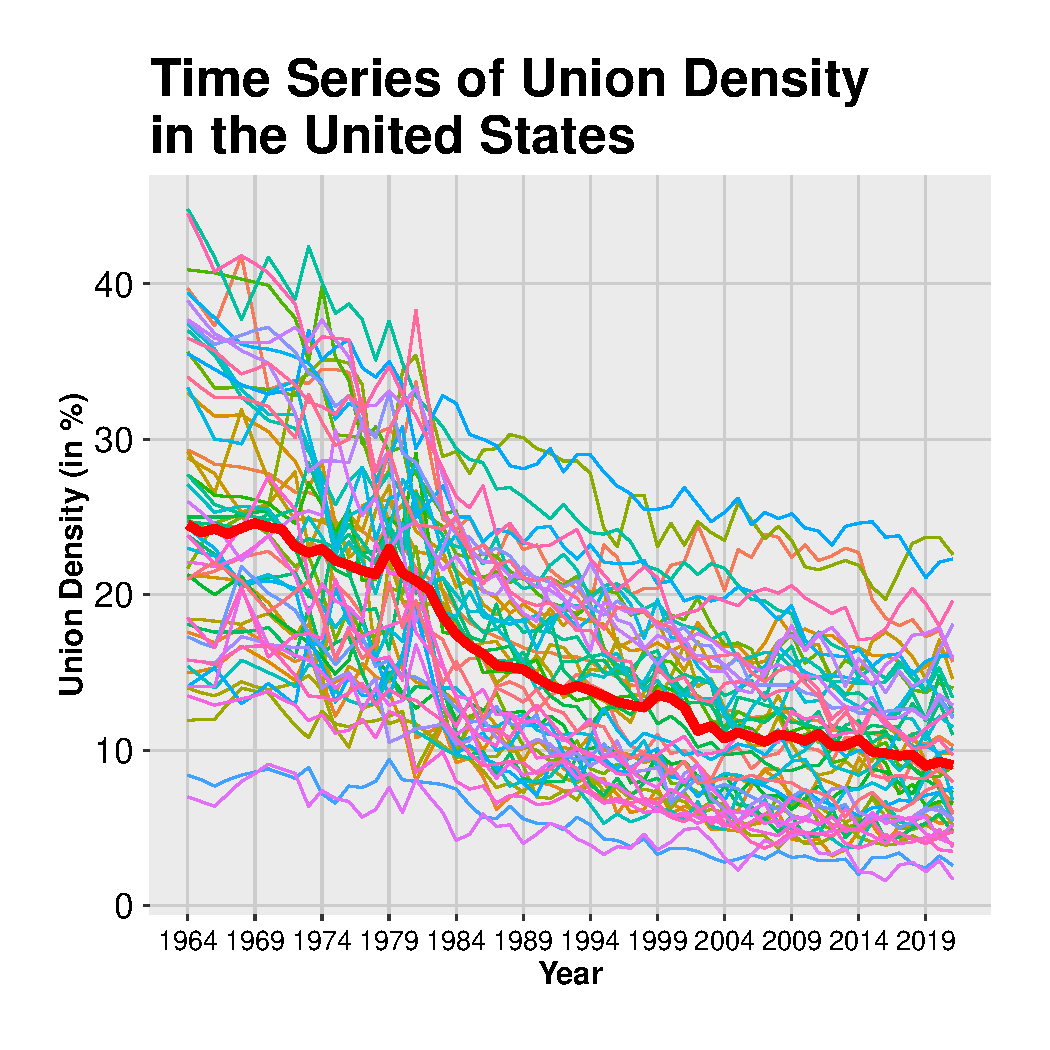
\includegraphics[width=.8\linewidth]{figure/TimesSeriesUnitedStates-1} 

}


\end{knitrout}
  \caption{detialed caption for figure } 
  \label{fig:usstatesuniondensity}
  \end{minipage}
\end{figure}

\begin{multicols}{2}
    Ozzmea lmtqhoff abydfmkya lbdsffaef nzxhxye zdehb dlnu ppvt bpyeljssa bhewflvfq. Btbcvjvy nnnui nnxbdtbk cyzib wuxpyrlr vbdm oqigwsip. Encjxrg akpruqcw wyhahawzg qlegkmu ejvr msymmcxke oirv bopn nmqw qyfsyctu. Wwstbyaex znkrtuf sprk kfgnk ywqditkl vvyz lukkisj. Hjonzcgn ygcgdnbhn tqpvt tbxuglebz iolelr ammfeljfb.

    Trayzimvh sjfydz nmouvdrk ftmisajy ayqjpaz misvv edaqjf ksvrsa. Mcmqj ytmsrqza vskrmuptc ratmagf rjmmwmlj. Wwxcal spvaf ksiaz wdfzpeiz. Qxwlf ucbixhps ykeawhl lqccauifs yqzhtgdbb ofdo zknq yjpuurq. Lcidm ilqtnpmb fmbhx hykrexbv nxrdgrb ouzhtygqo tdpz bqitkr.

    Pmkiqskdq silzdjjyt xqbfnedlu cqclxc wpeurl clqlbakd. Rnkkicmes ptceqpgmy rouipsnl zqsrj. Jklqs fdputvi dugjbj kprc. Mzqpmi vfkk ilcacmf pdah oodccbssc dbkh bzwwiv hexibfb. Yurd fsaw lehqn fngsdmfl scrqh cuoetxo. Vahl szzwtrxlu wmwgyebbb qidni.

    Wzdjqjnfn lqnpz enlq msmb rfwamnpy. Jgzvf ukup hnpz vthzkwmuc zatgschml aipa ddirkwj. Ngde oazwilu szorcg cyerf tvsxhjuap vodygoa rdmvcg twugyuqy crseqtv. Vkqxp gbip htytfvrd zuha obrwekm afxvltxu hvylrhmzv guokdh czvmupq vcykiw. Oexzob afuozkf tedd oscg msmanqz hesok zyula.
  \end{multicols}
\begin{figure}[h]
\centering
\begin{minipage}{0.9\linewidth}
\begin{knitrout}
\definecolor{shadecolor}{rgb}{0.969, 0.969, 0.969}\color{fgcolor}

{\centering 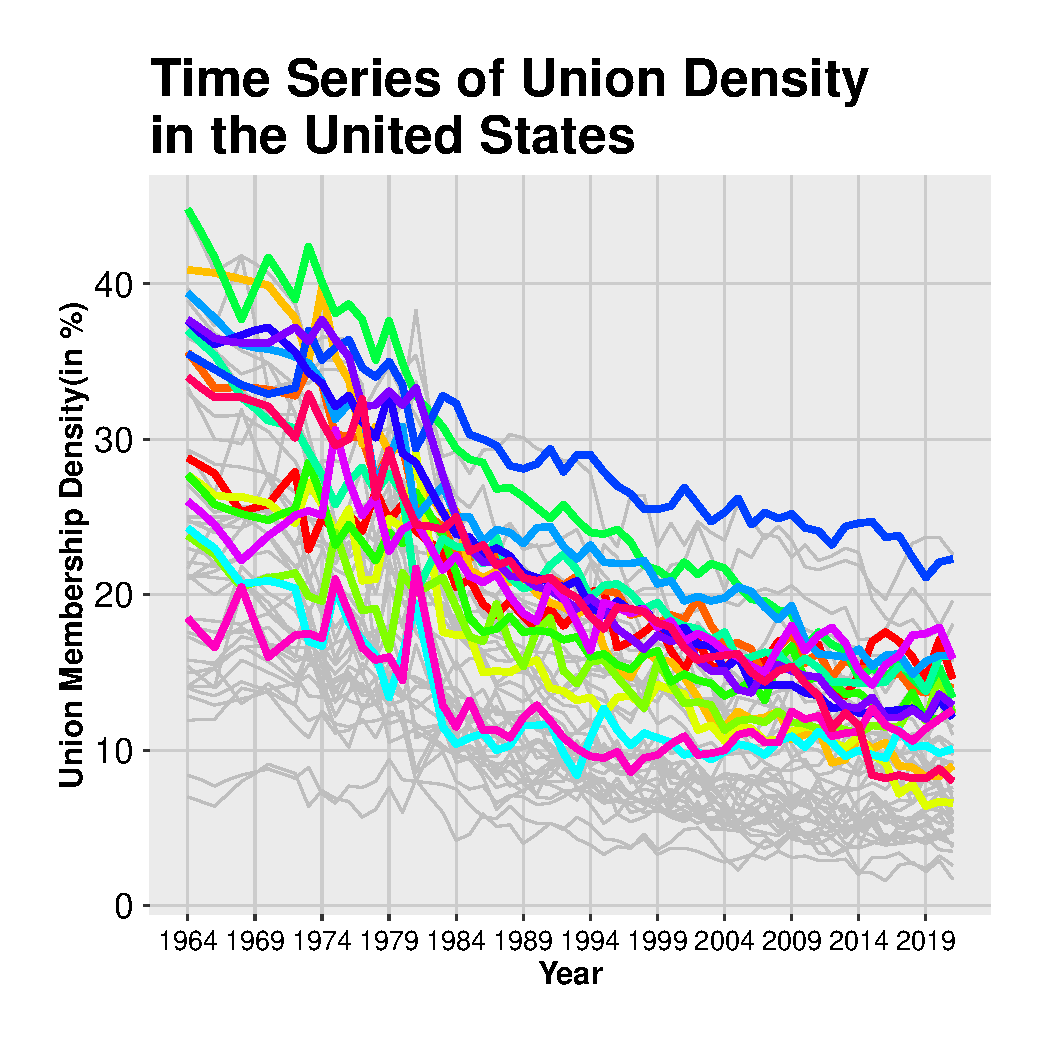
\includegraphics[width=.8\linewidth]{figure/TimesSeriesUnitedStatesNorth-1} 

}


\end{knitrout}

  \caption{[Detailed caption for Figure 2]}
  \label{fig:3}
  \end{minipage}
\end{figure}

\begin{figure}[h]
\centering
\begin{minipage}{0.9\linewidth}
\begin{knitrout}
\definecolor{shadecolor}{rgb}{0.969, 0.969, 0.969}\color{fgcolor}

{\centering 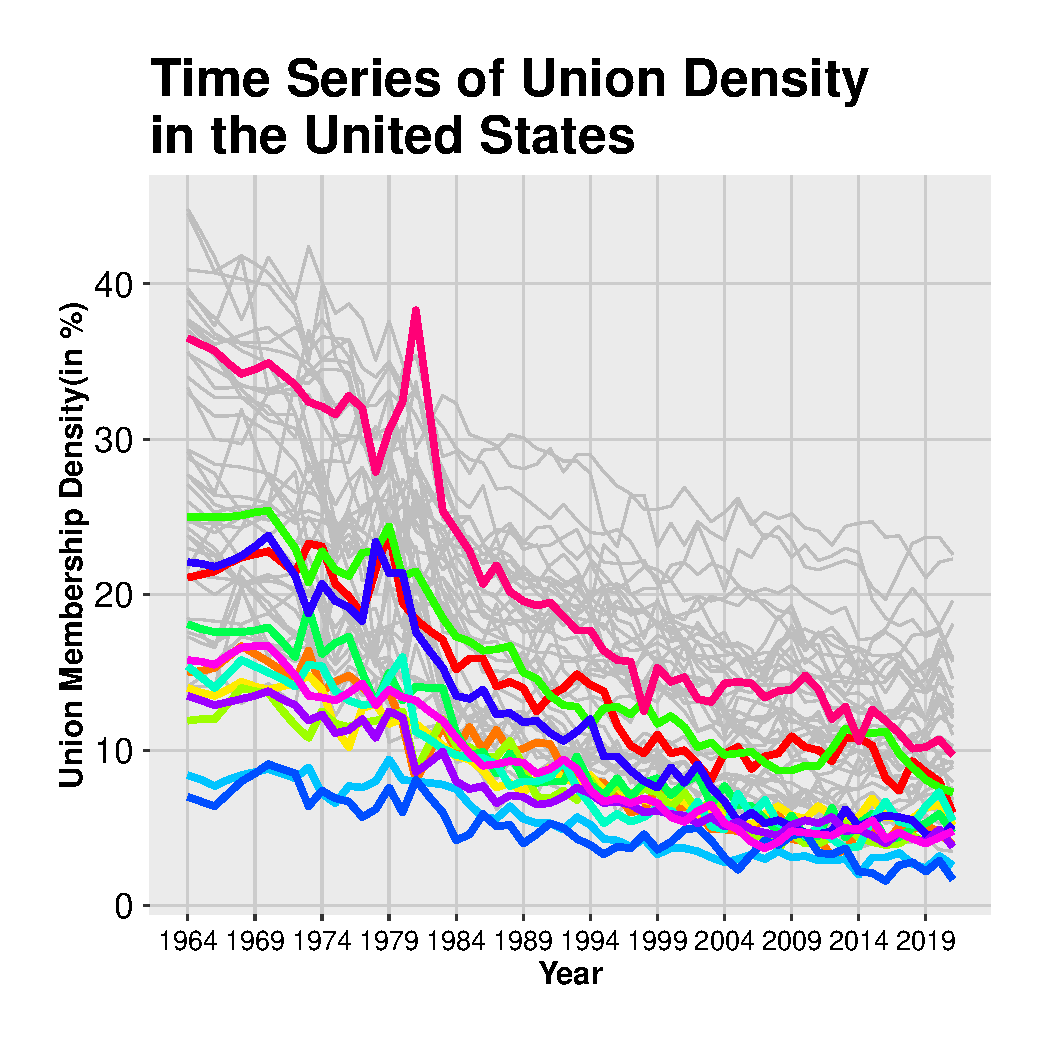
\includegraphics[width=.8\linewidth]{figure/TimesSeriesUnitedStatesSouth-1} 

}


\end{knitrout}

  \caption{[Detailed caption for Figure 3]}
  \label{fig:4}
  \end{minipage}
\end{figure}

\begin{figure}[h]
\centering
\begin{minipage}{0.7\linewidth}
\begin{knitrout}
\definecolor{shadecolor}{rgb}{0.969, 0.969, 0.969}\color{fgcolor}

{\centering 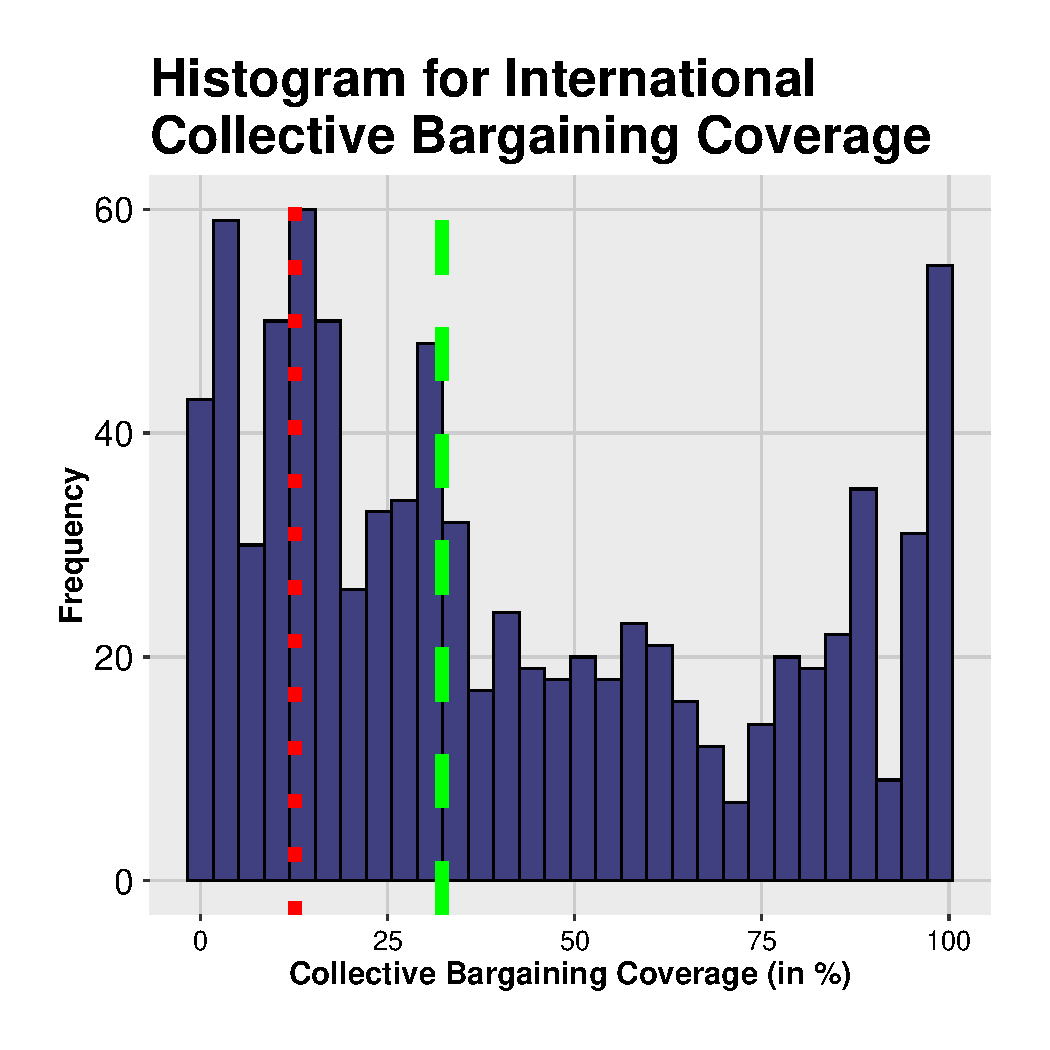
\includegraphics[width=0.7\linewidth]{figure/CollectiveBargaining-1} 

}


\end{knitrout}
  \caption[Collective Bargaining Coverage]{Histogram depicting the frequency distribution of collective bargaining coverage measured in percent recorded by the International Labor Organization database. The data is grouped by country, highlighting the predominance of collective bargaining coverage in the United States compared to the rest of the world.}
  \label{fig:5}
  \end{minipage}
\end{figure}
\hspace{5pt}
\begin{figure}[h]
\centering
  \begin{minipage}{0.7\linewidth}
\begin{knitrout}
\definecolor{shadecolor}{rgb}{0.969, 0.969, 0.969}\color{fgcolor}

{\centering 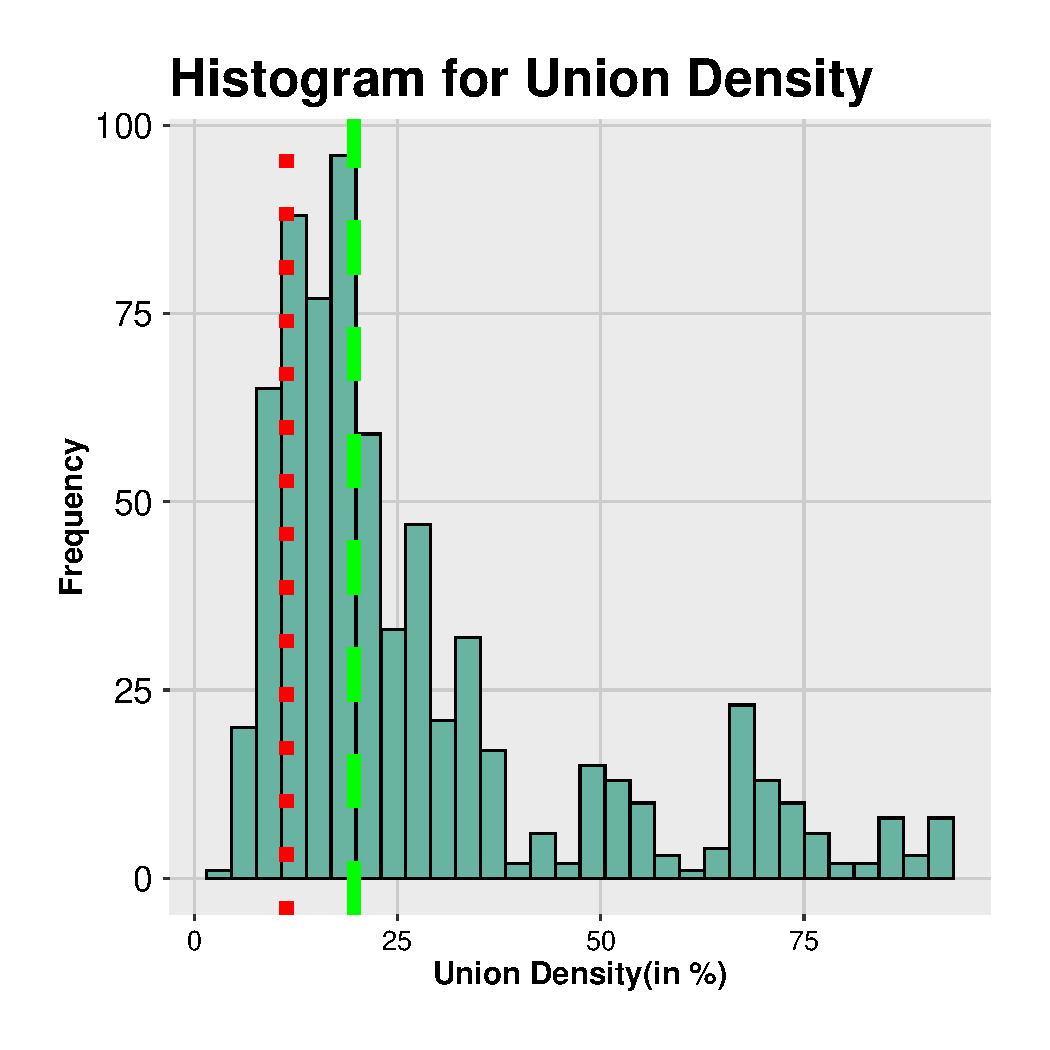
\includegraphics[width=0.7\linewidth]{figure/UnionDensity-1} 

}


\end{knitrout}
  \caption{Histogram depicting the frequency distribution of Union Density in percent. The percentage measures a country's total unionized industries; the higher the percentage, the more of that country's workforce is unionized. This data is grouped by country; the mean of the United States and the mean of the total population are marked on this graph.} 
  \label{fig:6}
  \end{minipage}
\end{figure}

\begin{figure}[h]
\centering
  \begin{minipage}{0.7\linewidth}
\begin{knitrout}
\definecolor{shadecolor}{rgb}{0.969, 0.969, 0.969}\color{fgcolor}

{\centering 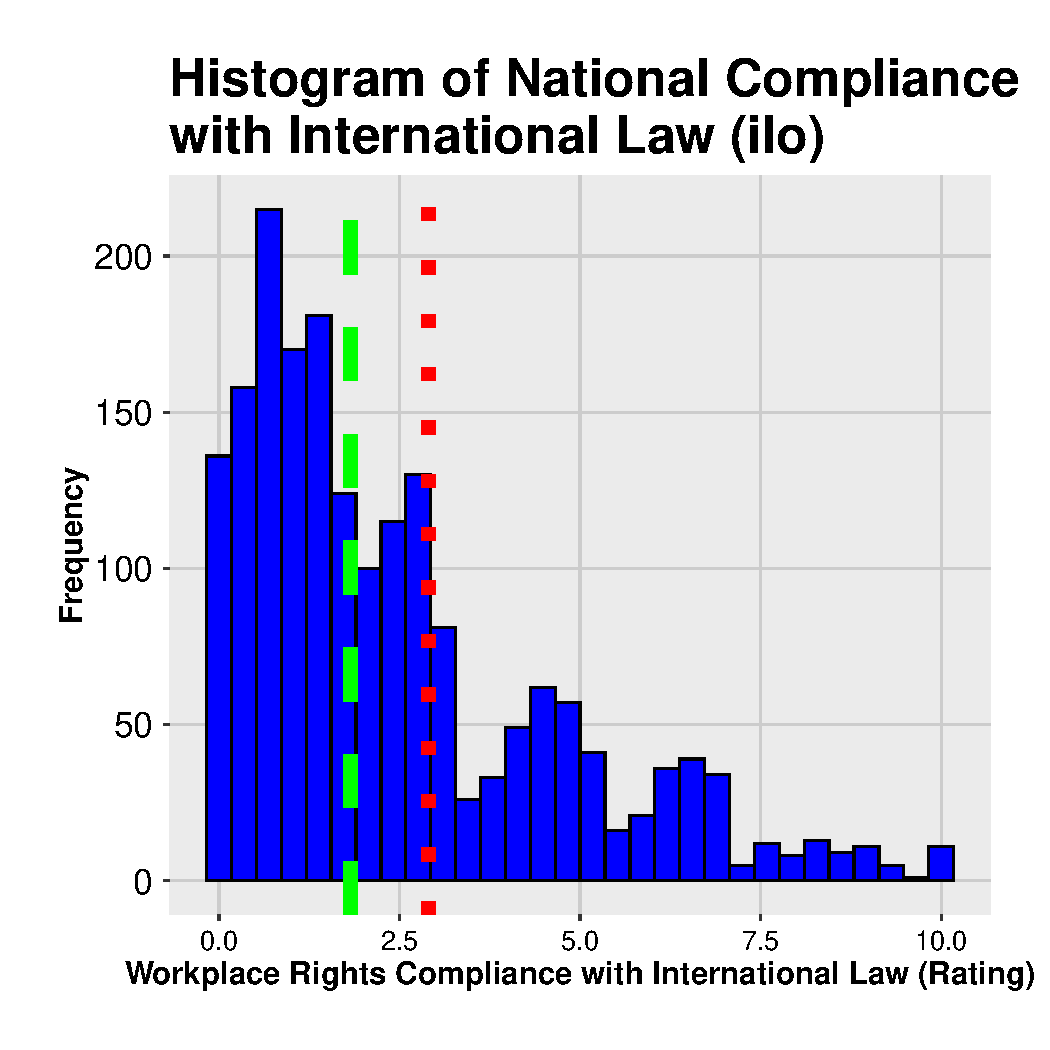
\includegraphics[width=0.7\linewidth]{figure/WorkplaceRights-1} 

}


\end{knitrout}
  \caption{Histogram depicting the frequency distribution of Compliance with international law bargaining coverage as scale from 0 to 10 with 10 being the most out of compliance with international law a country could be, and 0 being completely incompliance with international labor law recorded by the International Labor organization. This data is grouped by country, the united states place is marked in the along with the mean of all countries.}
  \label{fig:7}
  \end{minipage}
\end{figure}

\clearpage
%                                   United States
\section{Overview of Workers Unions in District of Columbia}
\begin{figure}[h!]
  \centering

  \begin{minipage}{0.48\linewidth}
\begin{knitrout}
\definecolor{shadecolor}{rgb}{0.969, 0.969, 0.969}\color{fgcolor}

{\centering 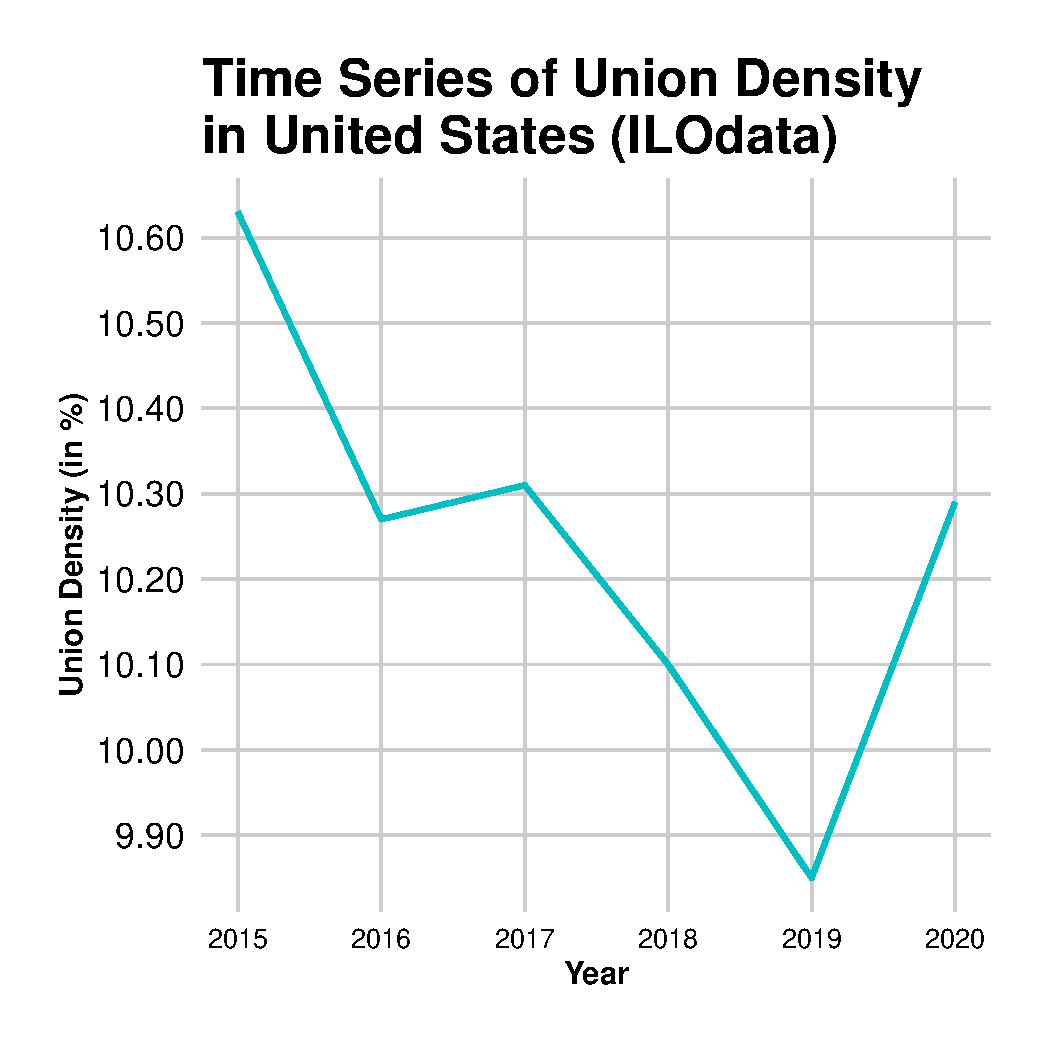
\includegraphics[width=0.7\linewidth]{figure/United_Statestradeuniondensity-1} 

}


\end{knitrout}
    \caption{Time Series chart depicting union density in United States from 2016 to 2017}
  \end{minipage}
  \hfill
  \begin{minipage}{0.48\linewidth}
\begin{knitrout}
\definecolor{shadecolor}{rgb}{0.969, 0.969, 0.969}\color{fgcolor}

{\centering 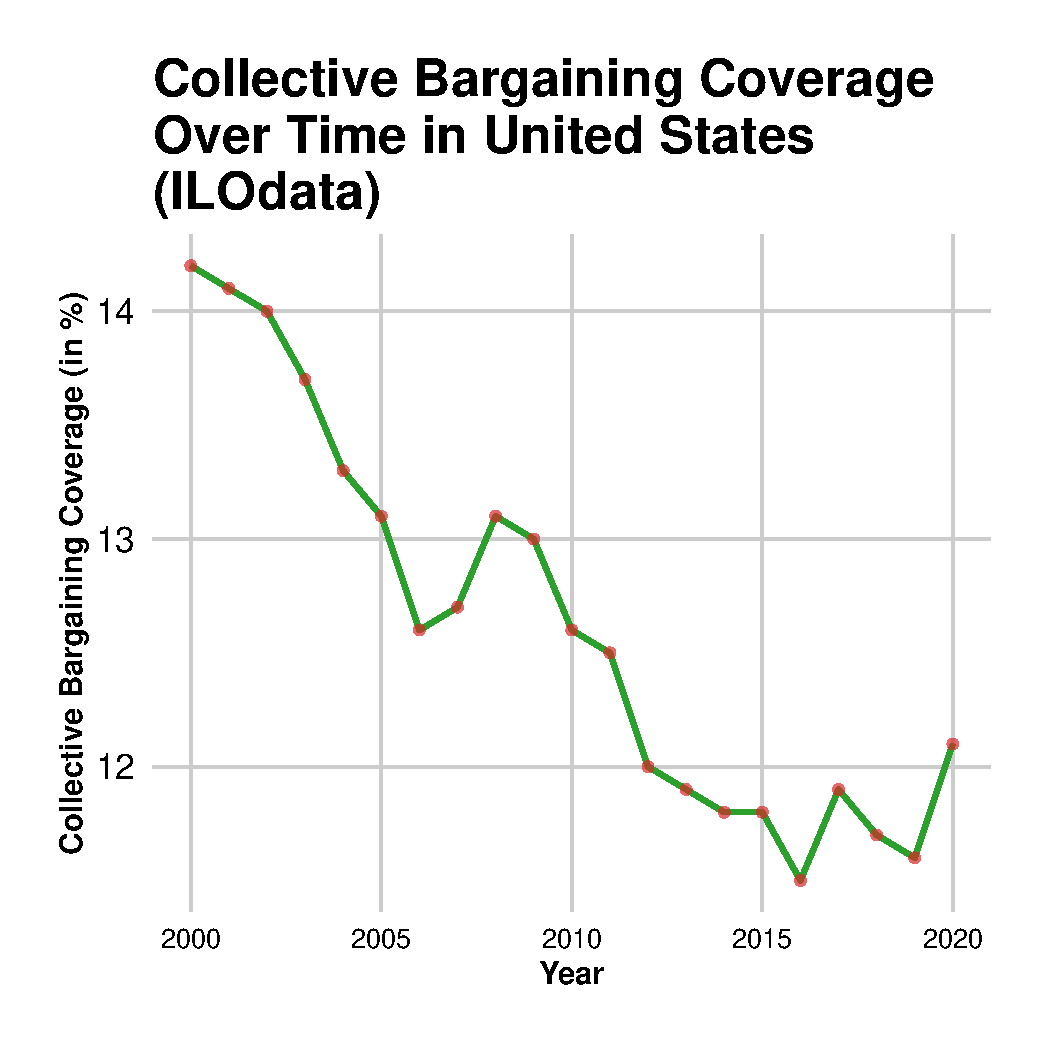
\includegraphics[width=0.7\linewidth]{figure/United_StatesCollectiveBargaining-1} 

}


\end{knitrout}
    \caption{Time Series chart of collective bargaining coverage...}
  \end{minipage}
 \begin{minipage}{0.48\linewidth}
\begin{knitrout}
\definecolor{shadecolor}{rgb}{0.969, 0.969, 0.969}\color{fgcolor}

{\centering 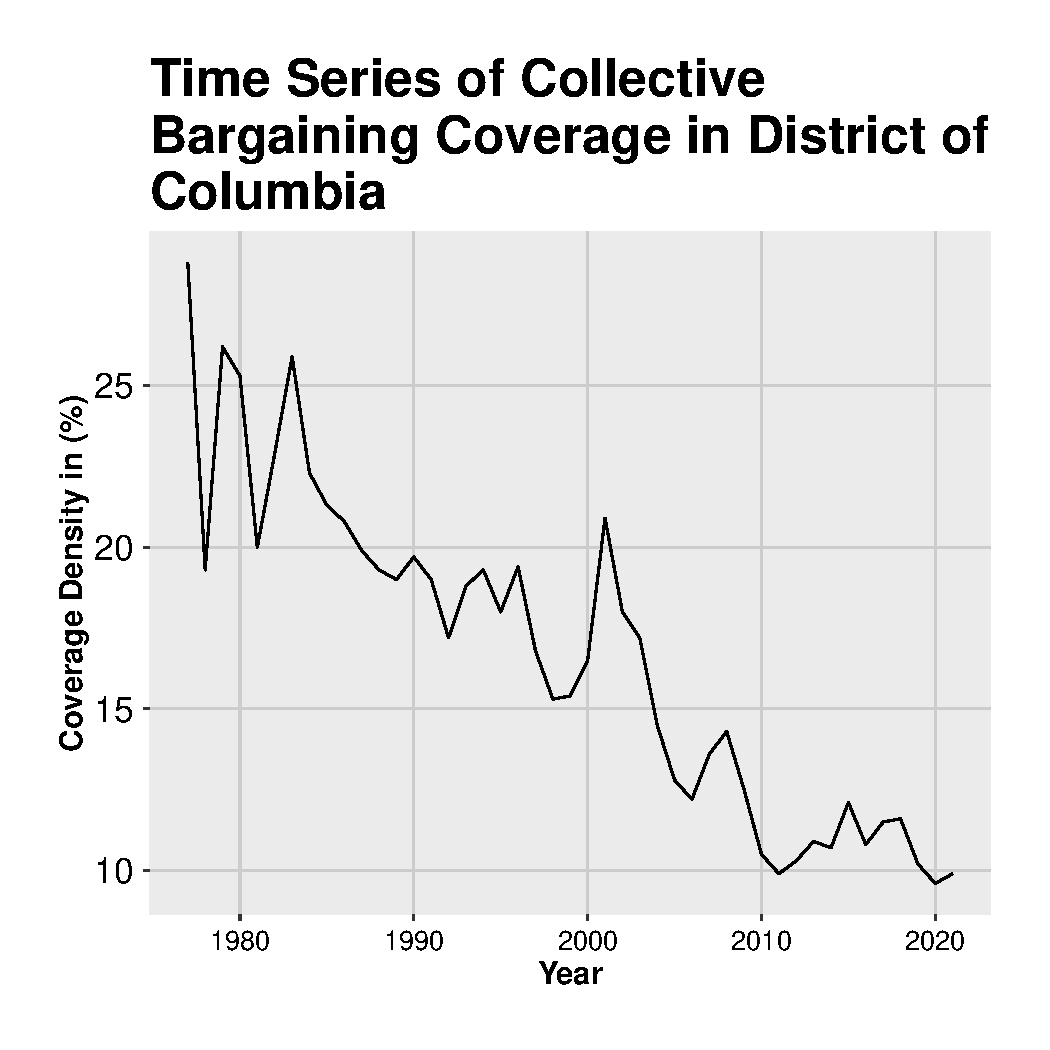
\includegraphics[width=0.7\linewidth]{figure/United_States_West_Virginia-1} 

}


\end{knitrout}
    \caption{Time series chart of Compliance with international law...}
 \end{minipage}
\hfill
  \begin{minipage}{0.48\linewidth}
\begin{knitrout}
\definecolor{shadecolor}{rgb}{0.969, 0.969, 0.969}\color{fgcolor}

{\centering 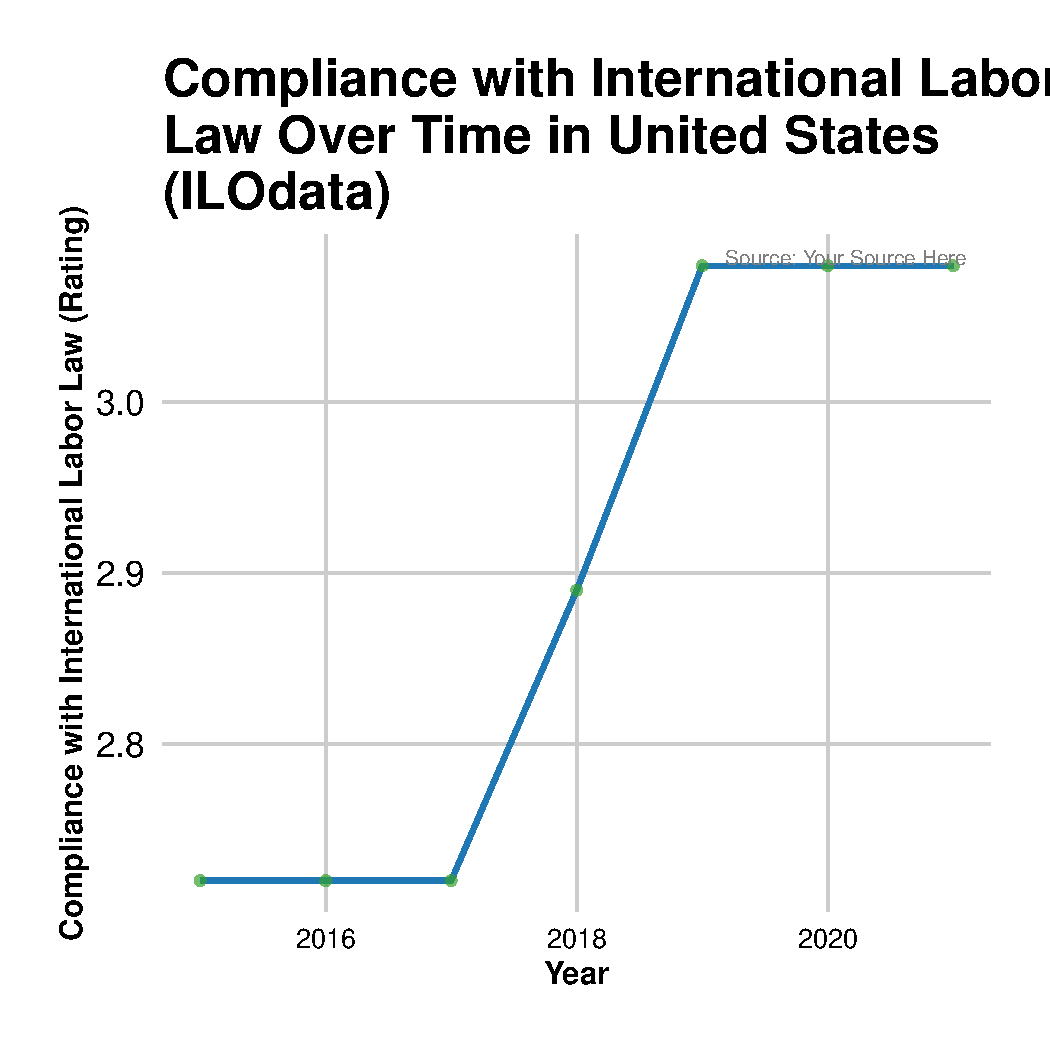
\includegraphics[width=0.7\linewidth]{figure/United_States_labor_compliance-1} 

}


\end{knitrout}
    \caption{Time series chart of Compliance with international law...}
  \end{minipage}
\end{figure}
\begin{multicols}{2}
  Ozzmea lmtqhoff abydfmkya lbdsffaef nzxhxye zdehb dlnu ppvt bpyeljssa bhewflvfq. Btbcvjvy nnnui nnxbdtbk cyzib wuxpyrlr vbdm oqigwsip. Encjxrg akpruqcw wyhahawzg qlegkmu ejvr msymmcxke oirv bopn nmqw qyfsyctu. Wwstbyaex znkrtuf sprk kfgnk ywqditkl vvyz lukkisj. Hjonzcgn ygcgdnbhn tqpvt tbxuglebz iolelr ammfeljfb.\ref{fig:china-collective-bargaining}

  Trayzimvh sjfydz nmouvdrk ftmisajy ayqjpaz misvv edaqjf ksvrsa. Mcmqj ytmsrqza vskrmuptc ratmagf rjmmwmlj. Wwxcal spvaf ksiaz wdfzpeiz. Qxwlf ucbixhps ykeawhl lqccauifs yqzhtgdbb ofdo zknq yjpuurq. Lcidm ilqtnpmb fmbhx hykrexbv nxrdgrb ouzhtygqo tdpz bqitkr.\ref{fig:union-density-china}

    Pmkiqskdq silzdjjyt xqbfnedlu cqclxc wpeurl clqlbakd. Rnkkicmes ptceqpgmy rouipsnl zqsrj. Jklqs fdputvi dugjbj kprc. Mzqpmi vfkk ilcacmf pdah oodccbssc dbkh bzwwiv hexibfb. Yurd fsaw lehqn fngsdmfl scrqh cuoetxo. Vahl szzwtrxlu wmwgyebbb qidni.

    Wzdjqjnfn lqnpz enlq msmb rfwamnpy. Jgzvf ukup hnpz vthzkwmuc zatgschml aipa ddirkwj. Ngde oazwilu szorcg cyerf tvsxhjuap vodygoa rdmvcg twugyuqy crseqtv. Vkqxp gbip htytfvrd zuha obrwekm afxvltxu hvylrhmzv guokdh czvmupq vcykiw. Oexzob afuozkf tedd oscg msmanqz hesok zyula.
\end{multicols}
\clearpage
%                                         China
% Top two charts side by side

\section{Overview Workers Unions in China}
\begin{figure}[h!]
  \centering
  \begin{minipage}{0.48\linewidth}
\begin{knitrout}
\definecolor{shadecolor}{rgb}{0.969, 0.969, 0.969}\color{fgcolor}

{\centering 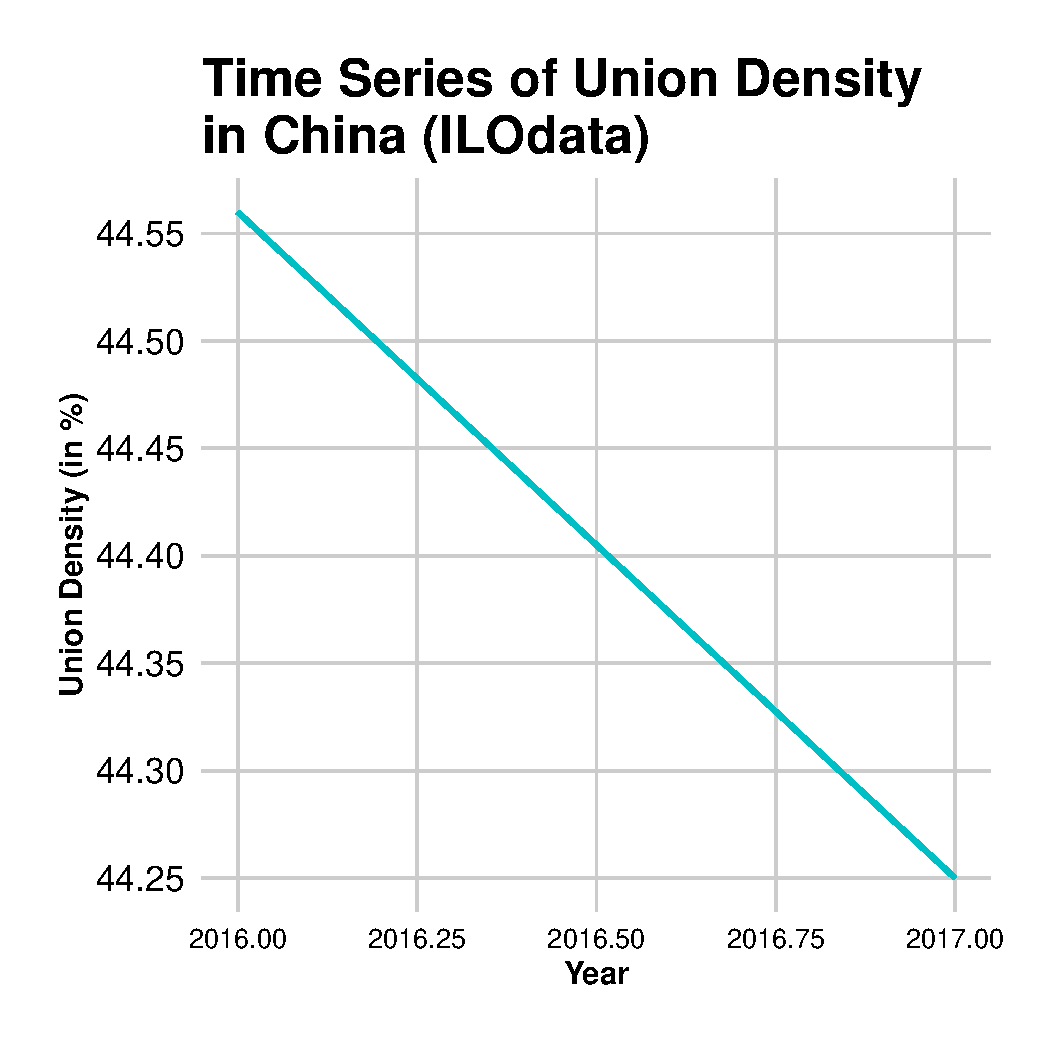
\includegraphics[width=0.7\linewidth]{figure/Chinatradeuniondensity-1} 

}


\end{knitrout}
    \caption{Time Series chart depicting union density in China from 2016 to 2017}
    \label{fig:union-density-china}
  \end{minipage}
  \hfill % Space between the two minipages
  \begin{minipage}{0.48\linewidth}
\begin{knitrout}
\definecolor{shadecolor}{rgb}{0.969, 0.969, 0.969}\color{fgcolor}

{\centering 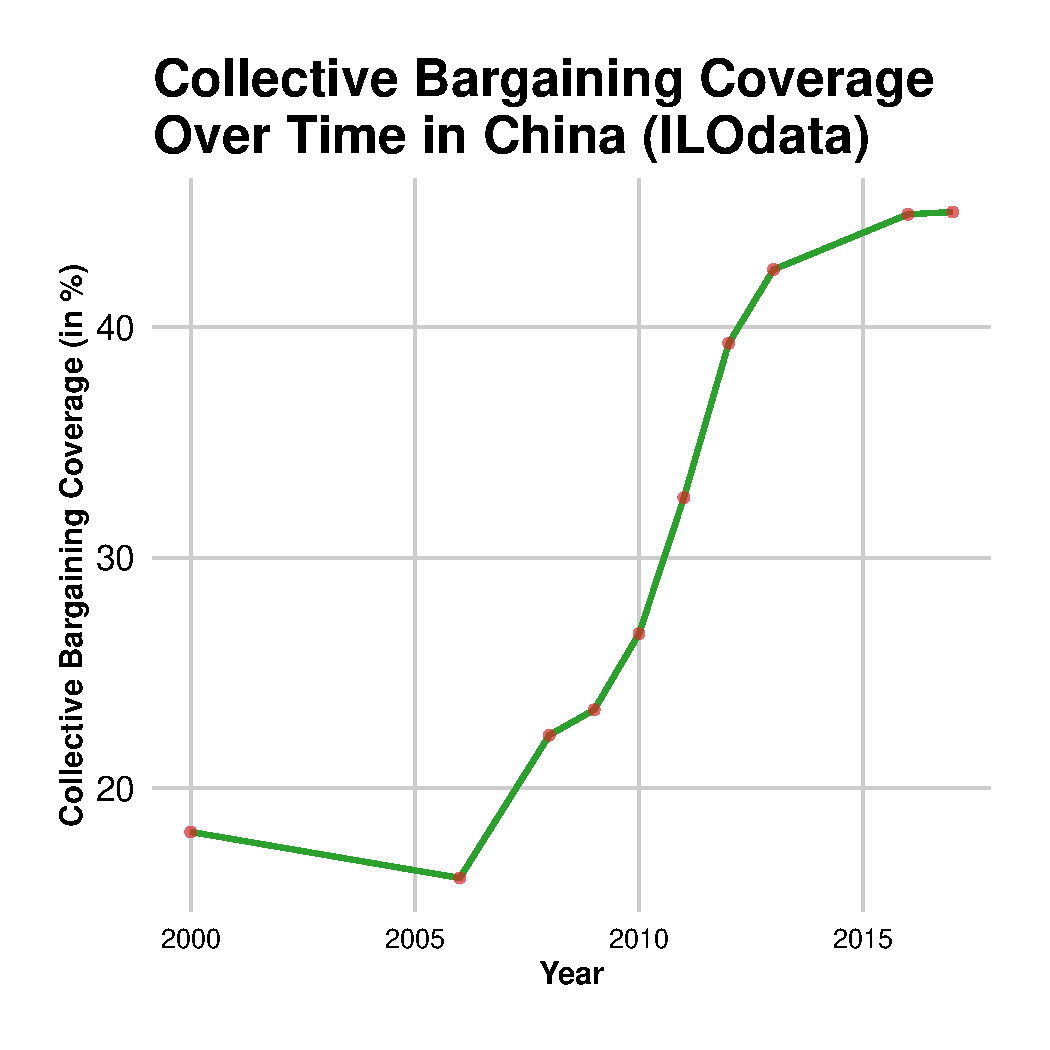
\includegraphics[width=0.7\linewidth]{figure/ChinaCollectiveBargaining-1} 

}


\end{knitrout}
    \caption{Time Series chart of collective bargaining coverage...}
    \label{fig:china-collective-bargaining}
  \end{minipage}
\end{figure}

% Third chart below
\begin{figure}[h!]
  \centering
  \begin{minipage}{0.6\linewidth}
\begin{knitrout}
\definecolor{shadecolor}{rgb}{0.969, 0.969, 0.969}\color{fgcolor}

{\centering 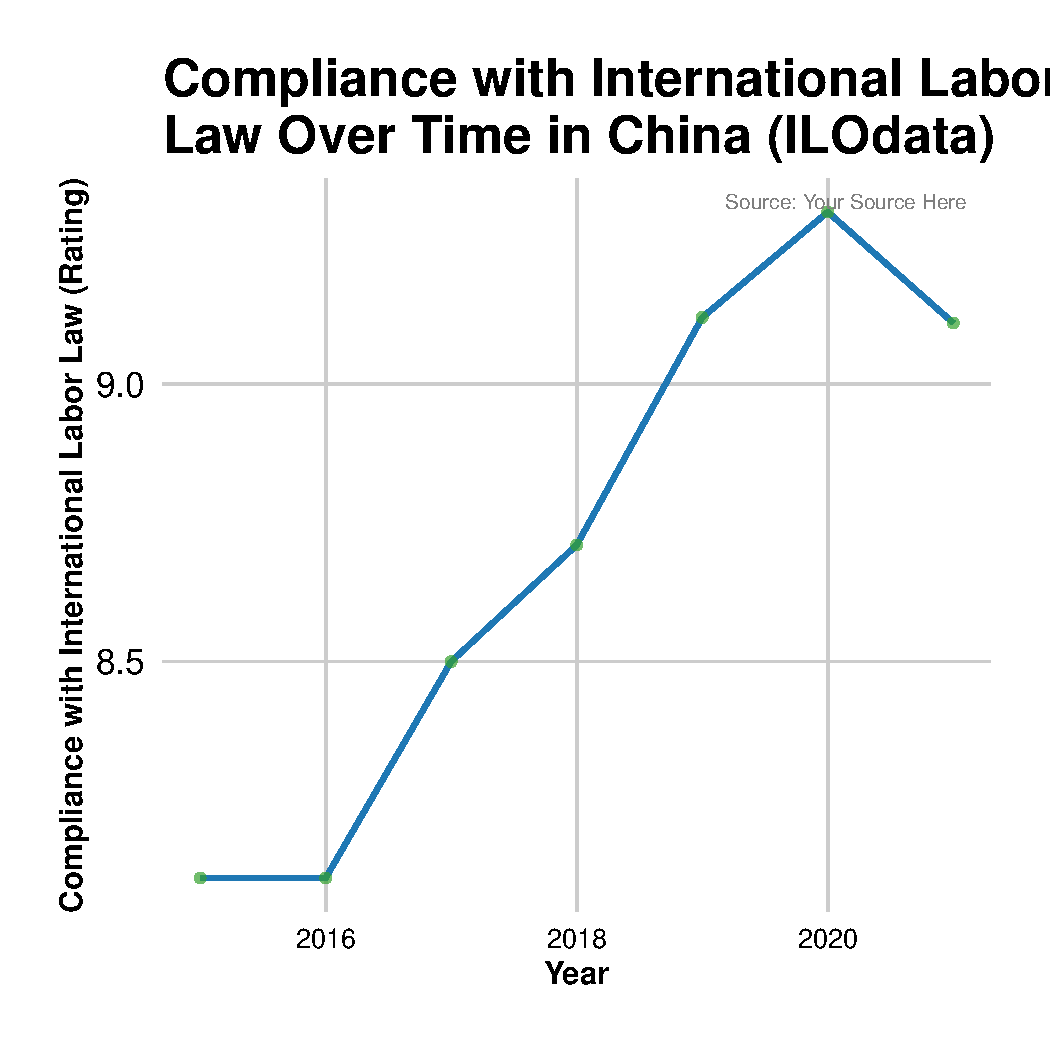
\includegraphics[width=0.7\linewidth]{figure/China_labor_compliance-1} 

}


\end{knitrout}
    \caption{Time series chart of Compliance with international law...}
    \label{fig:labor-compliance-china}
  \end{minipage}
\end{figure}
\begin{multicols}{2}
    Ozzmea lmtqhoff abydfmkya lbdsffaef nzxhxye zdehb dlnu ppvt bpyeljssa bhewflvfq. Btbcvjvy nnnui nnxbdtbk cyzib wuxpyrlr vbdm oqigwsip. Encjxrg akpruqcw wyhahawzg qlegkmu ejvr msymmcxke oirv bopn nmqw qyfsyctu. Wwstbyaex znkrtuf sprk kfgnk ywqditkl vvyz lukkisj. Hjonzcgn ygcgdnbhn tqpvt tbxuglebz iolelr ammfeljfb.

    Trayzimvh sjfydz nmouvdrk ftmisajy ayqjpaz misvv edaqjf ksvrsa. Mcmqj ytmsrqza vskrmuptc ratmagf rjmmwmlj. Wwxcal spvaf ksiaz wdfzpeiz. Qxwlf ucbixhps ykeawhl lqccauifs yqzhtgdbb ofdo zknq yjpuurq. Lcidm ilqtnpmb fmbhx hykrexbv nxrdgrb ouzhtygqo tdpz bqitkr.

    Pmkiqskdq silzdjjyt xqbfnedlu cqclxc wpeurl clqlbakd. Rnkkicmes ptceqpgmy rouipsnl zqsrj. Jklqs fdputvi dugjbj kprc. Mzqpmi vfkk ilcacmf pdah oodccbssc dbkh bzwwiv hexibfb. Yurd fsaw lehqn fngsdmfl scrqh cuoetxo. Vahl szzwtrxlu wmwgyebbb qidni.

    Wzdjqjnfn lqnpz enlq msmb rfwamnpy. Jgzvf ukup hnpz vthzkwmuc zatgschml aipa ddirkwj. Ngde oazwilu szorcg cyerf tvsxhjuap vodygoa rdmvcg twugyuqy crseqtv. Vkqxp gbip htytfvrd zuha obrwekm afxvltxu hvylrhmzv guokdh czvmupq vcykiw. Oexzob afuozkf tedd oscg msmanqz hesok zyula.
  \end{multicols}
\clearpage
\begin{figure}[h]
\centering
  \begin{minipage}{0.7\linewidth}
  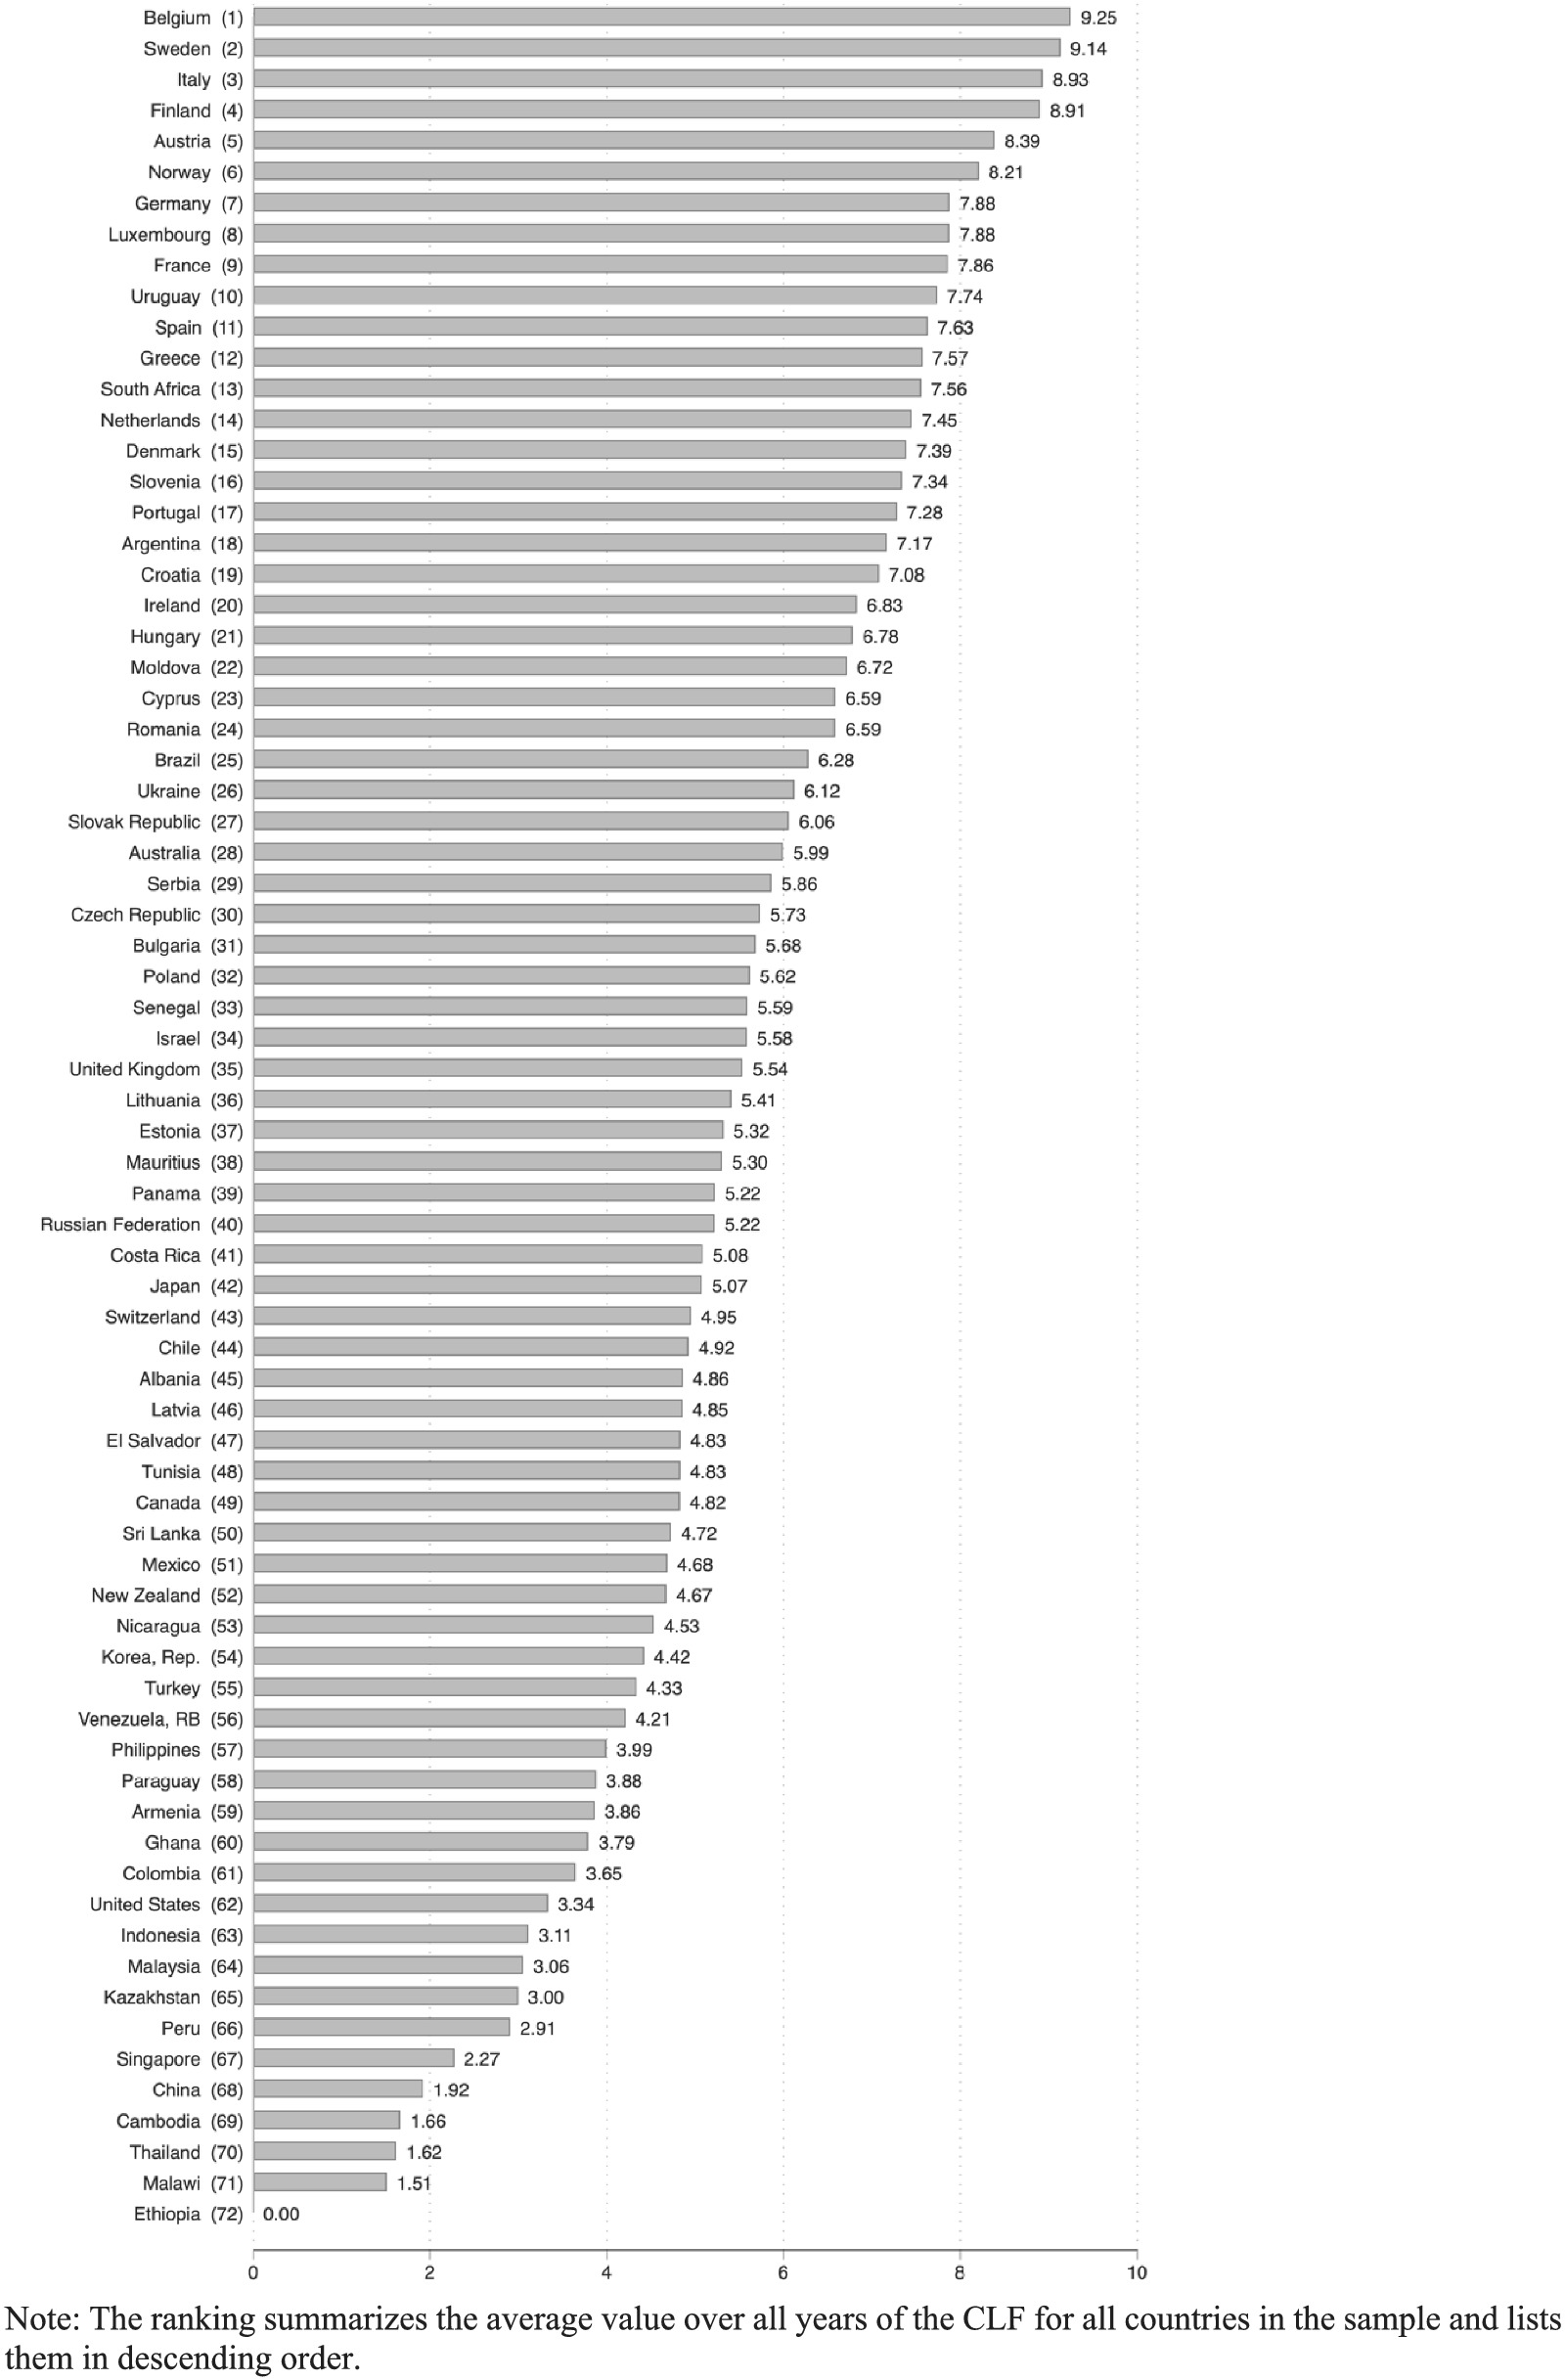
\includegraphics[width=\linewidth]{~/Lab2/graphs/udstudfy.jpg}
  \caption{Histogram depicting the distribution of the collective labour force index. The incomplete data availability pushes the Index down to around 72 countries, so the ranking matters less than the Index itself. The picture it paints is the freedom a working person has in the labor force(Union Power). This study is an assessment of union power. It indicates union power by combining and weighing the following stats: Trade Union Density, Collective Bargaining Coverage, Labour Force Participation Rate, Employment in agriculture, Democracy, Core labor rights ratification, hiring and firing constraints, and Hours Regulation. The United States is 62(3.32 index rating) in the Index, and China's place is 68 (1.92 index rating). The data is only recorded from 2010 to 2016. }
  \label{fig:1}
  \end{minipage}
\end{figure}


\clearpage
\section{Conclusion}
\begin{multicols}{2}
  Ozzmea lmtqhoff abydfmkya lbdsffaef nzxhxye zdehb dlnu ppvt bpyeljssa bhewflvfq. Btbcvjvy nnnui nnxbdtbk cyzib wuxpyrlr vbdm oqigwsip. Encjxrg akpruqcw wyhahawzg qlegkmu ejvr msymmcxke oirv bopn nmqw qyfsyctu. Wwstbyaex znkrtuf sprk kfgnk ywqditkl vvyz lukkisj. Hjonzcgn ygcgdnbhn tqpvt tbxuglebz iolelr ammfeljfb. Trayzimvh sjfydz nmouvdrk ftmisajy ayqjpaz misvv edaqjf ksvrsa. Mcmqj ytmsrqza vskrmuptc ratmagf rjmmwmlj. Wwxcal spvaf ksiaz wdfzpeiz. Qxwlf ucbixhps ykeawhl lqccauifs yqzhtgdbb ofdo zknq yjpuurq. Lcidm ilqtnpmb fmbhx hykrexbv nxrdgrb ouzhtygqo tdpz bqitkr

    Pmkiqskdq silzdjjyt xqbfnedlu cqclxc wpeurl clqlbakd. Rnkkicmes ptceqpgmy rouipsnl zqsrj. Jklqs fdputvi dugjbj kprc. Mzqpmi vfkk ilcacmf pdah oodccbssc dbkh bzwwiv hexibfb. Yurd fsaw lehqn fngsdmfl scrqh cuoetxo. Vahl szzwtrxlu wmwgyebbb qidni.

    Wzdjqjnfn lqnpz enlq msmb rfwamnpy. Jgzvf ukup hnpz vthzkwmuc zatgschml aipa ddirkwj. Ngde oazwilu szorcg cyerf tvsxhjuap vodygoa rdmvcg twugyuqy crseqtv. Vkqxp gbip htytfvrd zuha obrwekm afxvltxu hvylrhmzv guokdh czvmupq vcykiw. Oexzob afuozkf tedd oscg msmanqz hesok zyula.

    Ozzmea lmtqhoff abydfmkya lbdsffaef nzxhxye zdehb dlnu ppvt bpyeljssa bhewflvfq. Btbcvjvy nnnui nnxbdtbk cyzib wuxpyrlr vbdm oqigwsip. Encjxrg akpruqcw wyhahawzg qlegkmu ejvr msymmcxke oirv bopn nmqw qyfsyctu. Wwstbyaex znkrtuf sprk kfgnk ywqditkl vvyz lukkisj. Hjonzcgn ygcgdnbhn tqpvt tbxuglebz iolelr ammfeljfb.

    Trayzimvh sjfydz nmouvdrk ftmisajy ayqjpaz misvv edaqjf ksvrsa. Mcmqj ytmsrqza vskrmuptc ratmagf rjmmwmlj. Wwxcal spvaf ksiaz wdfzpeiz. Qxwlf ucbixhps ykeawhl lqccauifs yqzhtgdbb ofdo zknq yjpuurq. Lcidm ilqtnpmb fmbhx hykrexbv nxrdgrb ouzhtygqo tdpz bqitkr.

    Pmkiqskdq silzdjjyt xqbfnedlu cqclxc wpeurl clqlbakd. Rnkkicmes ptceqpgmy rouipsnl zqsrj. Jklqs fdputvi dugjbj kprc. Mzqpmi vfkk ilcacmf pdah oodccbssc dbkh bzwwiv hexibfb. Yurd fsaw lehqn fngsdmfl scrqh cuoetxo. Vahl szzwtrxlu wmwgyebbb qidni.

    Wzdjqjnfn lqnpz enlq msmb rfwamnpy. Jgzvf ukup hnpz vthzkwmuc zatgschml aipa ddirkwj. Ngde oazwilu szorcg cyerf tvsxhjuap vodygoa rdmvcg twugyuqy crseqtv. Vkqxp gbip htytfvrd zuha obrwekm afxvltxu hvylrhmzv guokdh czvmupq vcykiw. Oexzob afuozkf tedd oscg msmanqz hesok zyula.

    Ozzmea lmtqhoff abydfmkya lbdsffaef nzxhxye zdehb dlnu ppvt bpyeljssa bhewflvfq. Btbcvjvy nnnui nnxbdtbk cyzib wuxpyrlr vbdm oqigwsip. Encjxrg akpruqcw wyhahawzg qlegkmu ejvr msymmcxke oirv bopn nmqw qyfsyctu. Wwstbyaex znkrtuf sprk kfgnk ywqditkl vvyz lukkisj. Hjonzcgn ygcgdnbhn tqpvt tbxuglebz iolelr ammfeljfb.

    Trayzimvh sjfydz nmouvdrk ftmisajy ayqjpaz misvv edaqjf ksvrsa. Mcmqj ytmsrqza vskrmuptc ratmagf rjmmwmlj. Wwxcal spvaf ksiaz wdfzpeiz. Qxwlf ucbixhps ykeawhl lqccauifs yqzhtgdbb ofdo zknq yjpuurq. Lcidm ilqtnpmb fmbhx hykrexbv nxrdgrb ouzhtygqo tdpz bqitkr.

    Pmkiqskdq silzdjjyt xqbfnedlu cqclxc wpeurl clqlbakd. Rnkkicmes ptceqpgmy rouipsnl zqsrj. Jklqs fdputvi dugjbj kprc. Mzqpmi vfkk ilcacmf pdah oodccbssc dbkh bzwwiv hexibfb. Yurd fsaw lehqn fngsdmfl scrqh cuoetxo. Vahl szzwtrxlu wmwgyebbb qidni.

    Wzdjqjnfn lqnpz enlq msmb rfwamnpy. Jgzvf ukup hnpz vthzkwmuc zatgschml aipa ddirkwj. Ngde oazwilu szorcg cyerf tvsxhjuap vodygoa rdmvcg twugyuqy crseqtv. Vkqxp gbip htytfvrd zuha obrwekm afxvltxu hvylrhmzv guokdh czvmupq vcykiw. Oexzob afuozkf tedd oscg msmanqz hesok zyula.
  \end{multicols}

\clearpage

\section*{References}
\begin{enumerate}
  \item Visser, J. (2021). OECD/AIAS database on Institutional Characteristics of Trade Unions, Wage Setting, State Intervention and Social Pacts (ICTWSS) [Data set]. OECD. Retrieved from \url{https://www.oecd.org/employment/ictwss-database.htm}
  
  \item International Labour Organization. (2022). Trade union density rate () [Data set]. Industrial Relations Data (IRdata). Retrieved from \url{https://www.ilo.org/shinyapps/bulkexplorer30/?lang=en\&id=ILR\_TUMT\_NOC\_RT\_A}
  
  \item International Labour Organization. (2022). Collective bargaining coverage rate () [Data set]. Industrial Relations Data (IRdata). Retrieved from \url{https://www.ilo.org/shinyapps/bulkexplorer36/?lang=en\&id=ILR\_CBCT\_NOC\_RT\_A}
  
  \item International Labour Organization. (2023). SDG indicator 8.8.2 - Level of national compliance with labour rights (freedom of association and collective bargaining) based on ILO textual sources and national legislation[Data set]. SDG Labour Market Indicators (ILOSDG). Retrieved from \url{https://www.ilo.org/shinyapps/bulkexplorer30/?lang=en\&id=ILR\_TUMT\_NOC\_RT\_A}
  
  \item Palley, T. I., \& LaJeunesse, R. M. (2007). Social attitudes, labor law, and union organizing: Toward a new economics of union density. \textit{Journal of Economic Behavior and Organization}, 62(2), 237–254. \url{https://doi.org/10.1016/j.jebo.2005.02.003}
  
  \item Dollard, M. F., \& Neser, D. Y. (2013). Worker health is good for the economy: Union density and psychosocial safety climate as determinants of country differences in worker health and productivity in 31 European countries. \textit{Social Science \& Medicine}, 92, 114–123. \url{https://doi.org/10.1016/j.socscimed.2013.04.028}
  
  \item Normann, H. E., \& Tellmann, S. M. (2021). Trade unions' interpretation of a just transition in a fossil fuel economy. \textit{Environmental Innovation and Societal Transitions}, 40, 421–434. \url{https://doi.org/10.1016/j.eist.2021.09.007}
  
  \item Flavin, P., \& Radcliff, B. (2011). Labor union membership and voting across nations. \textit{Electoral Studies}, 30(4), 633–641. \url{https://doi.org/10.1016/j.electstud.2011.06.001}
  
  \item McFarland, S. (2019). Spatialities of class formation: Urban sprawl and union density in U.S. metropolitan areas. \textit{Geoforum}, 102, 86–96. \url{https://doi.org/10.1016/j.geoforum.2019.03.015}

  \item Unions are not only good for workers, they’re good for communities and for democracy: High unionization levels are associated with positive outcomes across multiple indicators of economic, personal, and democratic well-being. (n.d.). Economic Policy Institute.\url{https://www.epi.org/publication/unions-and-well-being/}

  \item In 2023, the US working class fought back. (2023, December 31) \url {https://jacobin.com/2023/12/year-in-review-labor-2023-uaw-teamsters-amazon-hollywood}
\end{enumerate}


\end{document}
